El tiempo de ejecución y uso de memoria medidos son registrados en archivos de texto. 
Con ayuda de los scripts \texttt{plotgenerator.py}, se generan los gráficos de los resultados, ejecutando “make plot”, definido en el \texttt{Makefile}.
\subsection*{Resultados Ordenamiento de Arreglos:}
Utilizando gráficos, se muestra los resultados principales obtenidos, comparando los tres algoritmos para distintos tipos de entradas. En el eje X se representa el Tamaño de entrada n, y en el eje Y se representa Tiempo de ejecución (ms), o uso de memoria (bytes), dependiendo del tipo de gráfico. \\

Se analizan todos los casos de prueba con datos ordenados de forma ascendente, aleatoria y descendente, con los que se obtiene los siguientes tiempos de ejecución promedio:\\
\begin{table}[ht]
  \centering
  \begin{tabular}{lrrrrr}
    Algoritmo  & MergeSort\.(ms) & QuickSort\.(ms)  & Sort\.(ms) \\
    10 & 0.003 & 0.001 & 0.0009\\
    1000 & 0.33 & 0.1 & 0.02\\
    100000 & 1505.27 & 568.85 & 1.33\\
    10 000 000 & - & - & -\\-
  \end{tabular}
  \caption{Tiempo de ejecución promedio para ordenamiento de arreglos}
  \label{tab:sorting-results}
\end{table}
Cabe notar que para 10.000.000 no hay datos medidos de tiempo de ejecución, ya que después de las 7 horas se detiene la ejecución, y se considera como caso outlier.\\
Es posible notar con el cuadro~\ref{tab:sorting-results}, que el algoritmo que en promedio se demora el mayor tiempo es \texttt{MergeSort}, y el algoritmo que es más eficiente es el \texttt{Sort}, de la librería C++.\\
\begin{figure}[H]
    \centering
      \begin{minipage}[t]{0.5\textwidth}
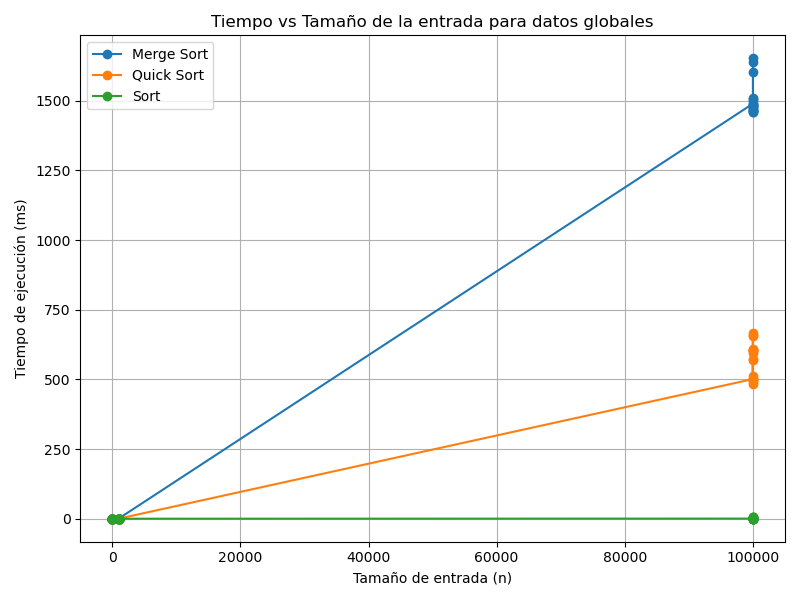
\includegraphics[width=\textwidth]{../code/sorting/data/plots/sorting_tiempo_comparacion.png}
      \end{minipage}%
      \begin{minipage}[t]{0.5\textwidth}
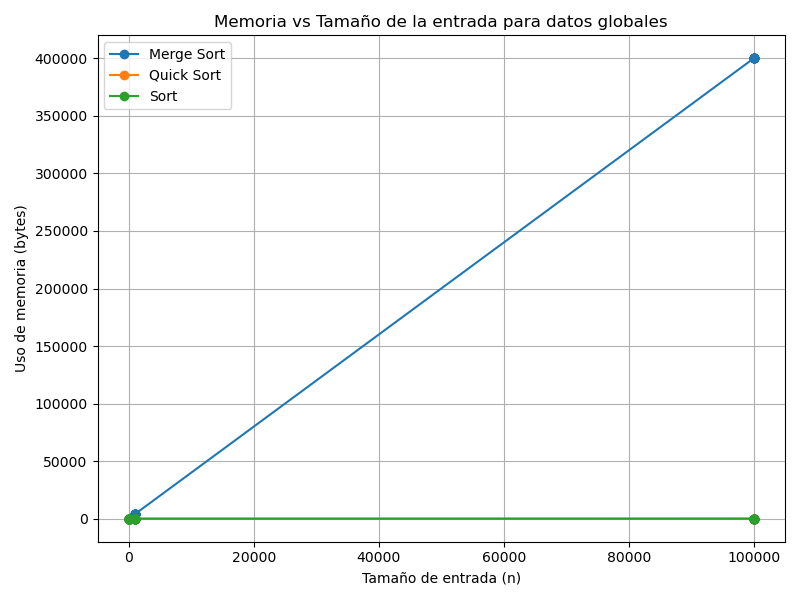
\includegraphics[width=\textwidth]{../code/sorting/data/plots/sorting_memoria_comparacion.png}
       \end{minipage}%
      \caption{Gráfico de tiempo de ejecución y uso de memoria para ordenamiento de arreglos.}
      \label{fig:sorting}
\end{figure}
Con los gráficos se puede notar que la memoria utilizada es igual para los algoritmos \texttt{QuickSort} y \texttt{Sort}. Además se corrobora lo mencionado sobre el cuadro~\ref{tab:sorting-results}, siendo \texttt{MergeSort} la curva con mayor tiempo, y \texttt{Sort}, la curva con tiempo más cercano a 0.

\newpage
\subsection*{Resultados Multiplicación de Matrices:}
Utilizando gráficos, se muestra los resultados principales obtenidos, comparando los dos algoritmos para distintos tipos de entradas. En el eje X se representa el Tamaño de la matriz ($n \times n$), y en el eje Y se representa Tiempo de ejecución (ms), o uso de memoria (bytes), dependiendo del tipo de gráfico. \\

Considerando todos los casos de prueba con matrices densas, dispersas y diagonales, se obtiene los siguientes tiempos de ejecución promedio:\\
\begin{table}[ht]
  \centering
  \begin{tabular}{lrr}
    Tamaño ($n \times n$)  & Naive\.(ms) & Strassen\.(ms)\\
    16 & 0.005 & 2.07\\
    64 & 0.26 & 114.23\\
    256 & 16.27 & 4493.9\\
    1024 & 1097.67 & 141855.75\\
  \end{tabular}
  \caption{Tiempos de ejecución promedio para Multiplicación de Matrices}
  \label{tab:mat-mult-results}
\end{table}
Se puede ver en la Tabla~\ref{tab:mat-mult-results}, que, el algoritmo que demora más tiempo es \texttt{Strassen}, y el algoritmo que demora menos es \texttt{Naive}.
\begin{figure}[H]
    \centering
    \begin{minipage}[t]{0.5\textwidth}
   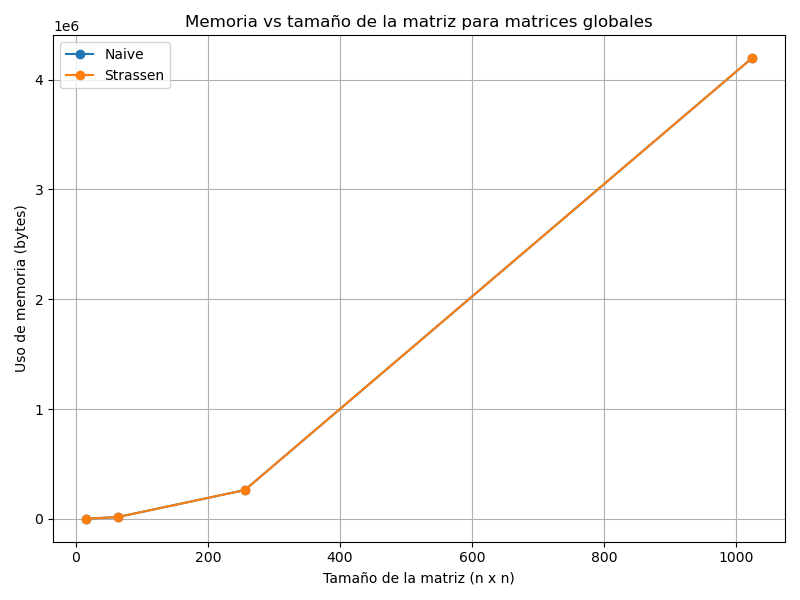
\includegraphics[width=\textwidth]{../code/matrix_multiplication/data/plots/matrix_memoria_comparacion.png}
    \end{minipage}%
    \begin{minipage}[t]{0.5\textwidth}
  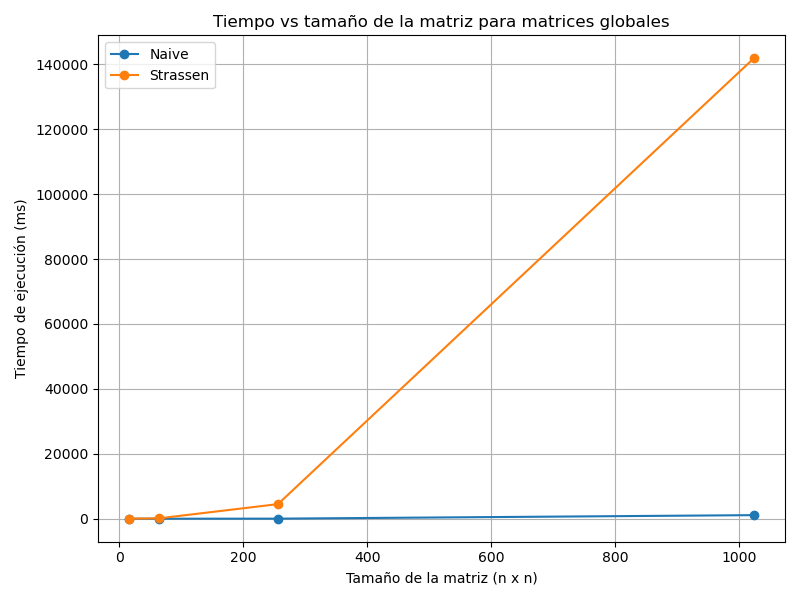
\includegraphics[width=\textwidth]{../code/matrix_multiplication/data/plots/matrix_tiempo_comparacion.png}
     \end{minipage}%
    \caption{Gráfico de tiempo de ejecución y uso de memoria para Multiplicación de Matrices.}
    \label{fig:mat-multi}
\end{figure}
Con los gráficos se puede notar que la memoria utilizada es igual para ambos algoritmos, y se corrobora lo mencionado sobre el cuadro~\ref{tab:mat-mult-results}, siendo \texttt{Strassen} la curva con mayor tiempo, y \texttt{Naive}, la curva con tiempo menor.